\documentclass[a4paper, 12pt, final, garamond]{book}
\usepackage{cours-preambule}

\begin{document}

\toggletrue{corrige}
\toggletrue{student}

Test switch normal~: \switch{student}{prof}
\smallbreak
Test switch corrig~: \cswitch{corrige}{enonce}

\bigbreak

Test switch imbriqués~:
\switch{
	\cswitch{student corrige}{student enonce}
}{
	\cswitch{prof corrige}{prof enonce}
}

\bigbreak

Test QR~:

\resetQ
\QR{Ceci est l'énoncé}{Ceci est le corrigé}

\begin{blocQR}
	\QR[2]{Q2}{E2}
	\QR[10]{Q3}{E3}
\end{blocQR}

\QR{Donner l'allure du graphe correspondant à $v(t)$.}{
	\begin{minipage}{0.49\linewidth}
		Le condensateur est initialement chargé. Soit $E$ sa tension initiale.
		On utilise l'équation 2 pour trouver que $\dv{v}{t} (0) =
			\frac{i' (0)}{C}$, sachant qu'à $t = 0$ le circuit est équivalent à un
		circuit $RC$ en décharge et qu'on a donc $i'(0) = E/R$. On trouve ainsi
		\[\boxed{\dv{v}{t} (0) = \frac{E}{\tau}}\]
		En finissant la détermination des constantes d'intégration, on trouve
		\begin{equation*}
			\boxed{v(t) = \frac{E}{\tau(r_+ - r_-)}
				\left[ \exr^{r_+t} - \exr^{r_-t} \right]}
		\end{equation*}
		\hfill
	\end{minipage}
	\begin{minipage}{0.49\linewidth}
		\begin{center}
			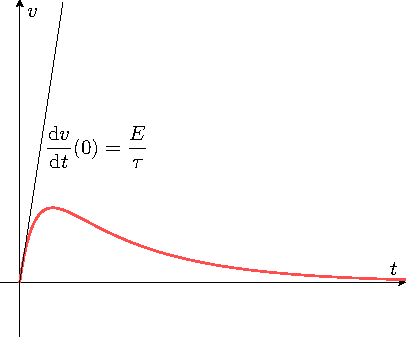
\includegraphics[width=\linewidth]{../2023/02_TD/02_elec/E4/figures/wien_carac}
		\end{center}
	\end{minipage}
}

\section{RLC échelon montant}

\begin{center}
	Indiquer la ou les bonnes réponses en justifiant tout votre raisonnement.
\end{center}

On considère un circuit RLC série, alimenté par une source idéale de tension de
force électromotrice $E$ constante comme schématisé ci-contre. Le condensateur
peut être court-circuité lorsque l'interrupteur K est fermé. On note $i(t)$
l'intensité du courant qui traverse la bobine et $u_C(t)$ la tension aux bornes
du condensateur C.

\begin{figure}[htbp]
	\centering
	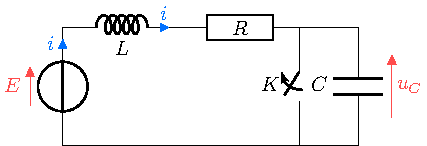
\includegraphics[width=.5\linewidth]{../2023/02_TD/02_elec/E4/figures/rlc_montant_switch}
\end{figure}

Le condensateur est mis en court-circuit par un interrupteur K depuis une durée
suffisamment longue, pour que le régime permanent soit établi. À l'instant pris
comme origine des temps, on ouvre l'interrupteur K.

\QR{Que valent l'intensité $i\left(0^+\right)$ et la tension $u_C(0^+)$ à
	l'instant $t=0^+$, succédant immédiatement à l'ouverture de l'interrupteur K~?
	Justifier tout votre raisonnement.
	\begin{tasks}[label=\protect\fbox{\Alph*}, label-width=4ex](4)
		\task $i\left(0^+\right)=0$
		\task $i\left(0^+\right)=\frac{E}{R}$
		\task $u_C\left(0^+\right)=0$
		\task $u_C\left(0^+\right)=E$
	\end{tasks}%
}
{ Intéressons-nous d'abord au circuit à $t<0$. L'interrupteur est alors fermé si
	bien que $u_C$ est une tension aux bornes d'un fil donc
	\[
		u_C\left(t=0^-\right)=0
	\]
	De plus, le condensateur assure la continuité de la tension à ses bornes,
	donc
	\[
		u_C\left(t=0^+\right)=u_C\left(t=0^-\right)=0
	\]
	Par ailleurs en régime permanent constant, on sait que la bobine est
	équivalente à un interrupteur fermé (un fil). Si bien que le circuit est alors
	équivalent à uniquement la résistance $R$ en série avec la source idéale de
	fem $E$. Ainsi d'après la loi de Pouillet,
	\[
		i\left(t=0^-\right)=E/R
	\]
	De plus, la bobine assure la continuité de l'intensité qui la traverse, donc
	\[
		i\left(t=0^+\right)=i\left(t=0^-\right)=\frac{E}{R}
	\]
	Réponses B et 42.
}



\end{document}
